\documentclass[twocolumn]{article}

\usepackage{amsmath}
\usepackage{siunitx}
\usepackage{xcolor}
\usepackage{titling}
\usepackage{graphicx}
\usepackage{booktabs}
\usepackage{tabularx}
\usepackage{enumitem}
\usepackage{lmodern}
% \usepackage{placeins}
% \usepackage{hhline}
\usepackage{ctex}
\usepackage{siunitx}
% \usepackage{biblatex}
\usepackage{hyperref}

\newcolumntype{A}{>{\centering\arraybackslash}X}
\newcolumntype{B}{>{\centering\arraybackslash\bfseries}X}
\definecolor{mydarkblue}{rgb}{0,0.08,0.45}
\hypersetup{%
  pdftitle={蜗壳 365},
  pdfauthor={张学涵},
  pdfsubject={余庆杯项目报告},
  pdfkeywords={蜗壳大雾实验工具, 蜗壳排课工具, 我的科大, 程序设计, 团队协作},
  pdfborder=0 0 0,
  pdfpagemode=UseNone,
  colorlinks=true,
  linkcolor=mydarkblue,
  citecolor=mydarkblue,
  filecolor=mydarkblue,
  urlcolor=mydarkblue,
}
\title{%
蜗壳 365\\
\large 余庆杯项目报告}
\setlength{\droptitle}{-1.2in}
\posttitle{\par\end{center}\vspace{-0.2in}}
\preauthor{}
\postauthor{}
\author{}
\predate{}
\postdate{}
\date{}
% \addbibresource{main.bib}

\begin{document}

\twocolumn[\maketitle
\begin{tabularx}{\textwidth}{|A|A|A|}
\hline
队长 & 孙旭磊 & PB21000270 \\
\hline
队员1 & 赵奕 & PB21000033 \\
\hline
队员2 & 张学涵 & PB21000079 \\
\hline
子项目 & \multicolumn{2}{c|}{大雾实验工具 \& 蜗壳排课工具 \& 我的科大APP} \\
\hline
\end{tabularx}
\vskip .2in
\vskip\baselineskip]
\section{项目需求分析}

\subsection{大雾实验工具}

大物实验在\href{https://icourse.club/course/12716/}{评课社区}、\href{https://www.zhihu.com/question/35867101}{知乎}等网站上一直饱受争议,
有多名同学指出实验报告撰写耗时长、专业作图软件难以使用、Word 中打数学公式麻烦等问题。
鉴于此,曾经有学长在开发过一款\href{https://github.com/regymm/PhysicsExp}{大物实验数据处理工具},
这是非常好的创意。但是,这款软件入门成本太高,故了解它的人很少。

本小组开发的\href{https://dawu.feixu.site/}{\emph{大雾实验工具}}是一款网页应用,无需安装任何软件,更不需要有编程基础,没有任何学习成本。
本工具的目标用户是中国科学技术大学大一本科生,着力于解决其撰写实验报告时最耗时的三件事情,即“绘制图像”“计算不确定度”“在电脑上书写公式”。

当然,一些高级软件也能出色地完成上述的本工具的功能,如专业绘图软件 Origin, 专业计算软件 Matlab 等。
但我们的项目不是去取代这些强大的软件,而是将它们\emph{本地化}。
这些软件功能繁多,故学习成本相对较高,但我们的软件为每一个大物实验都写了专门的处理工具,封装到只需要用户上传数据表格的程度。
相比动辄几个 \unit{\giga\byte} 的专业软件来说,我们的工具更加友好,更加便捷,更加有针对性——更加有效。

\subsection{蜗壳排课工具}

每个学期的选课前夕,学生们总是细心地筹划他们的理想课程表。为了成功挑选出自己喜爱的课程,他们往往付出许多时间和力气来避免课程之间的时间冲突。在 Excel 表格中,他们反复调整,时而将某个课程替换为另一个课程。

本小组开发的\href{https://paike.feixu.site/}{\emph{蜗壳排课工具}}也是一款网页应用,致力于解决同学们的这一难题。

\subsection{我的科大 APP}

科大的网络资源虽然丰富,但由于网站分布散乱。我们在各种 QQ 群中常常看到有人寻找各种网站的链接。
而\href{https://myustc.feixu.site/}{\emph{我的科大}}将常用的科大网站汇聚一处,点击即可直接访问。

然而,科大大部分的网站并未针对小屏幕设备进行优化,导致在手机上阅读时经常需要进行缩放才能清晰看见文字。在某些浏览器上,元素重叠的问题甚至导致无法点击功能键。
为了解决这个问题,我们的软件进行了深度改造以适应手机浏览,从而使得包括课程表、考试信息等页面在手机上的浏览体验大幅度提升。
更为便利的是,这些页面可以直接查看,无需登录教务系统,快速方便。学生们还可以创建桌面快捷方式,实现从系统桌面直接访问。
\section{项目功能设计}

\subsection{蜗壳大雾实验工具}

\subsubsection{总体功能说明}

本工具通过腾讯云服务器搭建于网页平台,支持任何设备自由访问。
传入实验数据后,本工具立刻完成绘制图像、计算不确定度、生成计算公式等一系列操作,
并将最终结果整理成一份 Word 文档,下载后即可直接使用。
本实验工具支持一级大物的 25 个实验,如图 \ref{fig:main} 所示,这大大提升了学生们撰写实验报告的效率。
由于本工具只是将传入的实验数据进行自动分析,故其不会造成抄袭、造假等学术不端问题。

\begin{figure}[p]
  \centering
  
\includegraphics[height=0.95\textheight]{figure/main.png}
  \caption{大雾实验工具网站主界面}
  \label{fig:main}
\end{figure}

\subsubsection{具体功能点说明}

使用本工具时,用户只需输入他们做实验时测量到的原始数据,
而无需任何额外的计算处理,用户所要做的只有按照规定的格式上传 Excel 文档。
本工具支持 \verb|xlsx|, \verb|csv| 等各种格式的数据表格。
具体而言,每个实验都会有一张示例数据表供用户参考,如图 \ref{fig:interface} 的界面所示。
用户也可以直接下载示例数据,并直接在它的基础上进行修改。
因此,本工具没有任何学习成本,是一款即点即用、免安装的简单轻应用。

\begin{figure}[p]
  \centering
  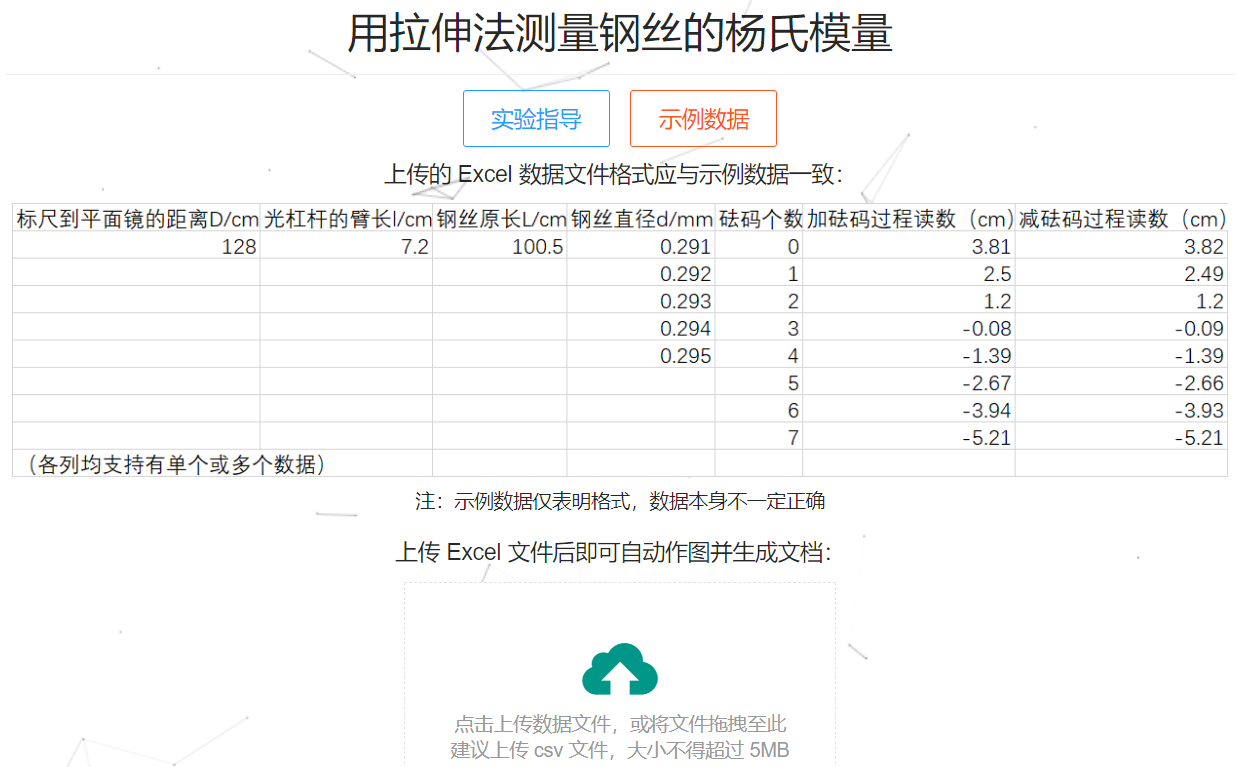
\includegraphics[width=0.67\columnwidth]{figure/interface.png}
  \caption{“拉伸法测钢丝杨氏模量”的工具界面}
  \label{fig:interface}
\end{figure}

另外,本工具贴心地提供了不确定度表格与通用的计算工具,并且每个实验都附有可在线浏览的实验指导。

{\noindent\bfseries\textbullet{}绘制图像}

本工具根据输入的数据以及实验原理,自动生成美观的实验图像,
支持平滑去噪、数据拟合、双 y 图等多种图像生成需求,如图 \ref{fig:draw} 所示。

\begin{figure}[p]
  \centering
  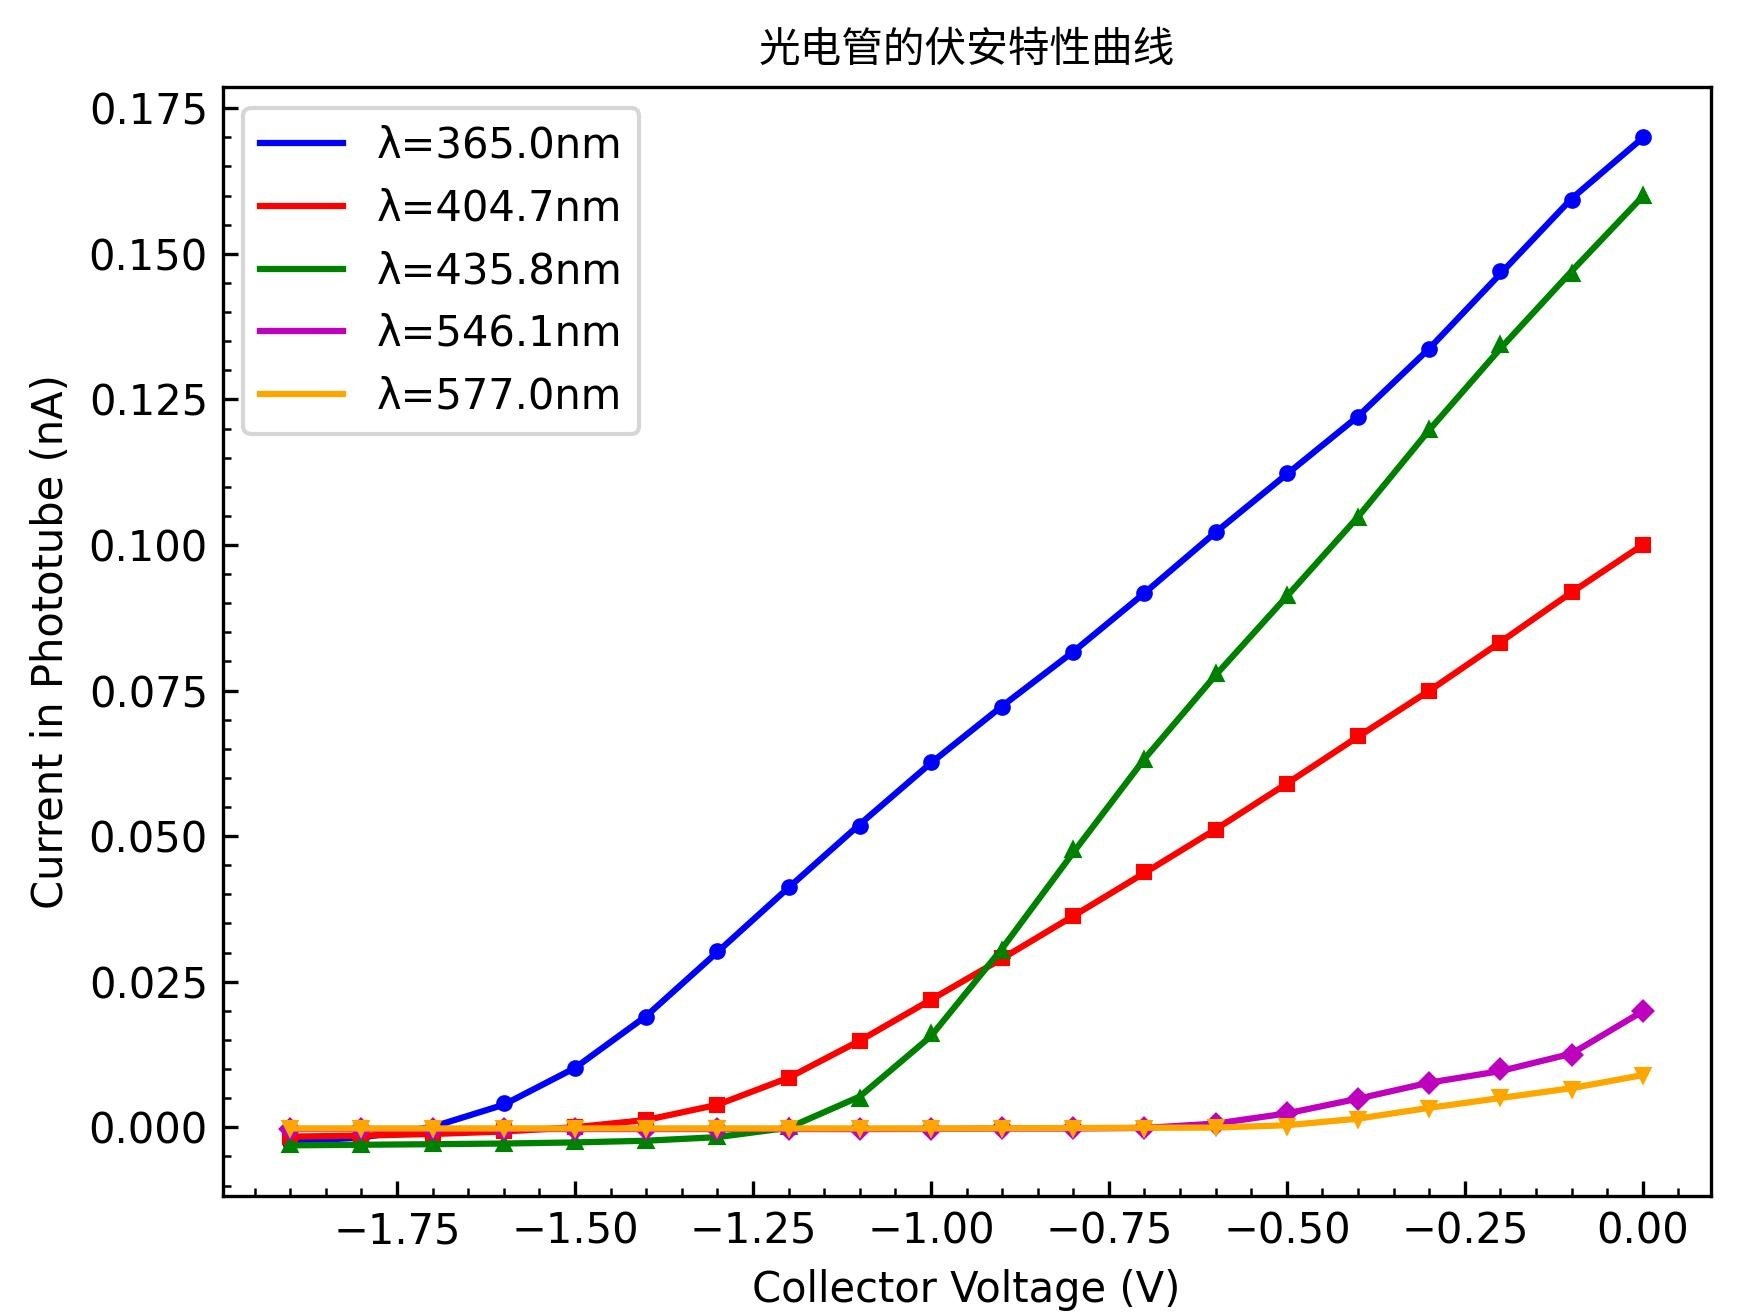
\includegraphics[width=0.67\columnwidth]{figure/draw.jpg}
  \caption{平滑连接的光电效应伏安特性曲线}
  \label{fig:draw}
\end{figure}

{\noindent\bfseries\textbullet{}计算不确定度与生成计算公式}

本工具在生成的 Word 文档中渲染了各种公式,如图 \ref{fig:calc} 所示。
用户可以直观看到不确定度每一步的计算过程,并在自己的报告中直接使用这些算式与结果。

\begin{figure}[p]
  \centering
  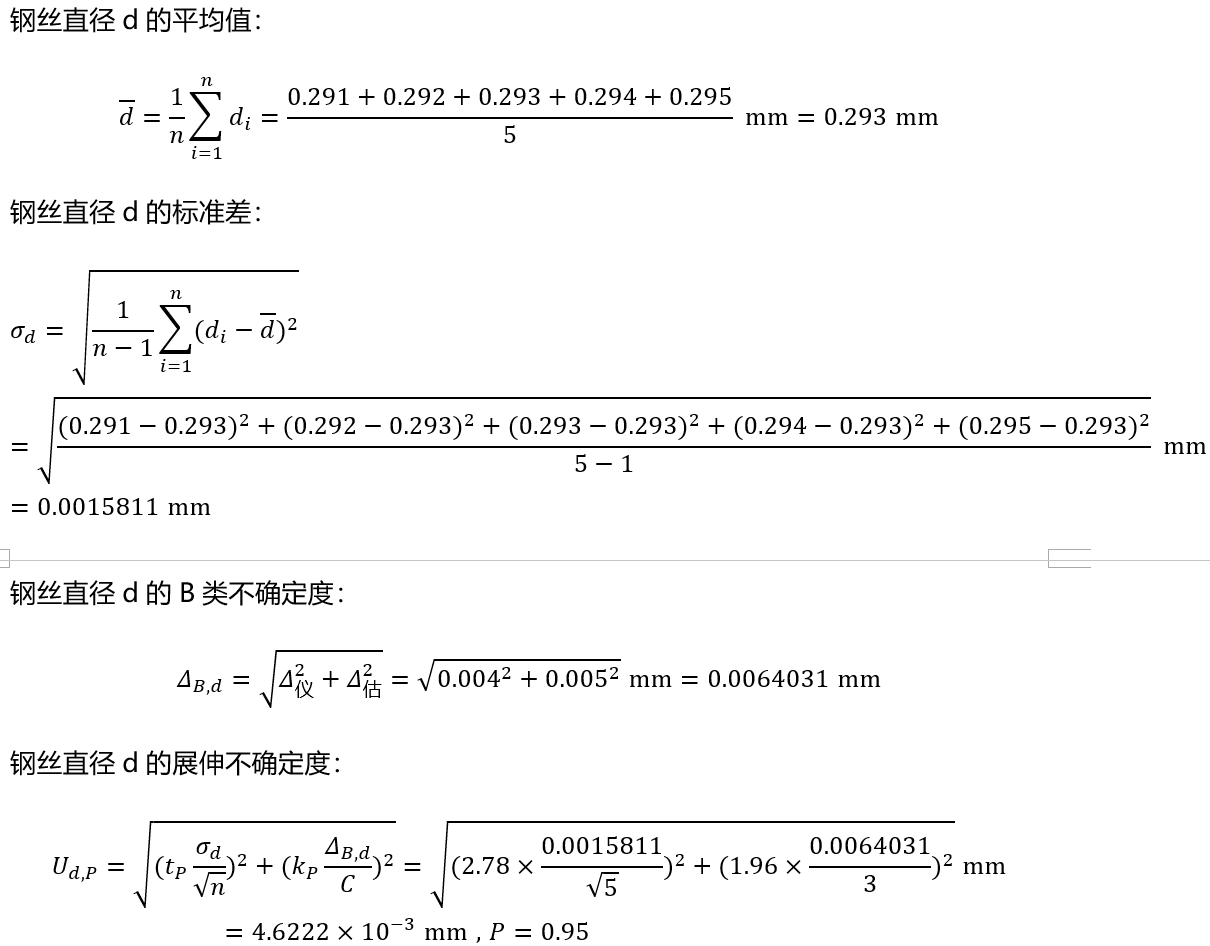
\includegraphics[width=0.67\columnwidth]{figure/calc.png}
  \caption{不确定度计算的详细过程}
  \label{fig:calc}
\end{figure}

在 Word 文档中除了有已经渲染好的公式外,
我们还提供了它们的 \LaTeX{} 源码,如图 \ref{fig:latex} 所示。
这极大方便了用 \LaTeX{}, Markdown 等排版实验报告的用户,使他们无需手动敲入每一个算式。

\begin{figure}[htbp]
  \centering
  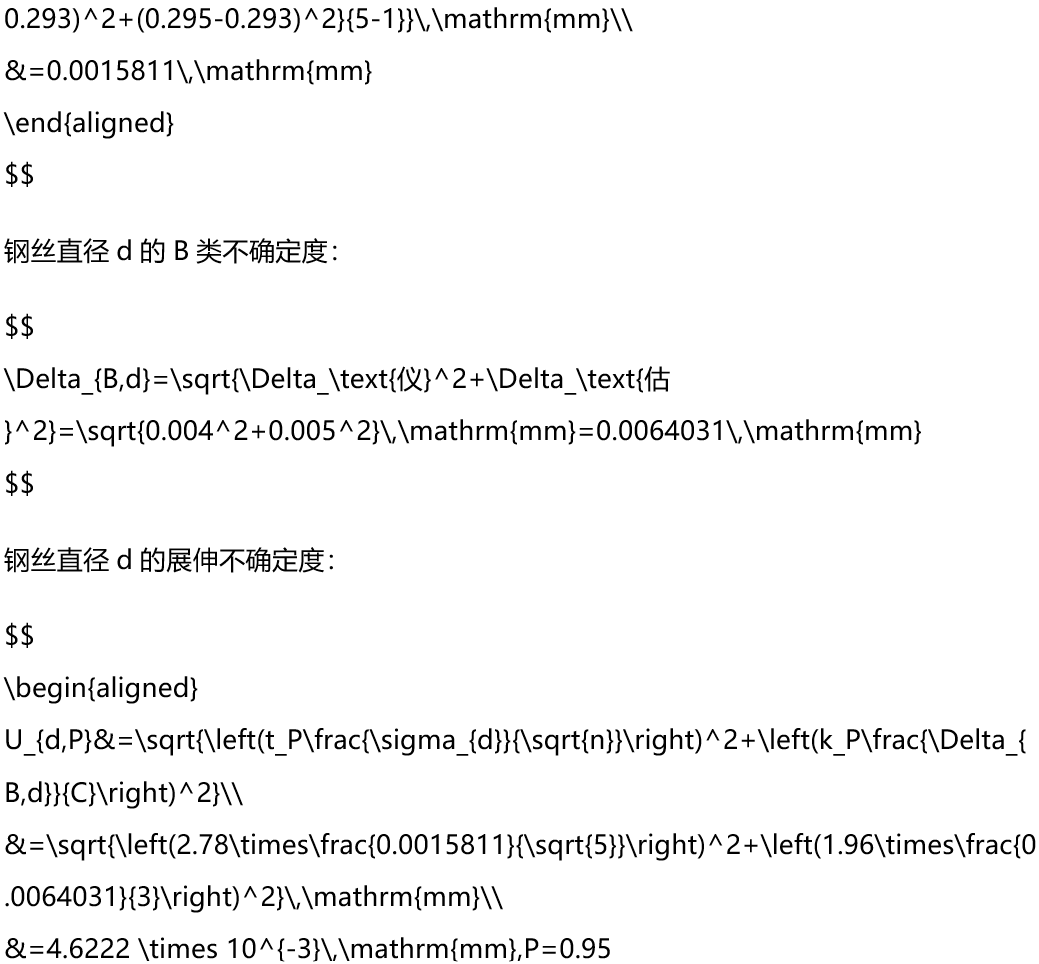
\includegraphics[width=0.67\columnwidth]{figure/latex.png}
  \caption{不确定度算式的 \LaTeX{} 源码}
  \label{fig:latex}
\end{figure}

\subsubsection{功能点设计细节}

本工具后端使用 Python 编写,使用的包与模块如表 \ref{tab:pkg} 所示。
前端由 HTML 编写,并使用了 \verb|Flask| Web 应用框架。以下将详细介绍各功能的实现,分为图像绘制、数据处理和文档生成三部分。

\begin{table}[htbp]
  \caption{本工具使用的全部 Python 包与模块}
  \label{tab:pkg}
  \vskip 0.1in
  \centering\small
  \begin{tabular}{lc}
  \toprule
  Python 包或模块 & 用途 \\
  \midrule
  \verb|chardet| & 检测用户上传的数据表格的编码 \\
  \verb|collections| & 通过 \verb|namedtuple| 使代码更清晰 \\
  \verb|Flask| & Web 应用框架 \\
  \verb|latex2mathml| & \LaTeX{} 代码转换为 \verb|MathML| 代码 \\
  \verb|lxml| & \verb|MathML| 代码转 \verb|Office MathML| \\
  \verb|math|, \verb|numpy| & 不确定度数字运算 \\
  \verb|Matplotlib| & 绘制物理图像 \\
  \verb|os|, \verb|random|, \verb|shutil| & 后台文件操作与管理 \\
  \verb|pandas| & 数据表格处理 \\
  \verb|python-docx| & 生成 Word 文档 \\
  \verb|SciPy| & 数据拟合 \\
  \verb|SymPy| & 不确定度符号运算 \\
  \verb|time|, \verb|threading| & 定时删除生成的 Word 文档 \\
  \verb|traceback| & 打印运行错误以便调试 \\
  \bottomrule
  \end{tabular}
  \vskip -0.1in
\end{table}

\subsubsection{图像绘制}

图像由 \verb|Matplotlib| 绘制。我们的规范如下:
\begin{itemize}
  \item 面向绘图对象作图:\verb|fig, ax = matplotlib|\\\verb|.pyplot.subplots()|
  \item 设置副刻度为主刻度的一半,主刻度为默认:\verb|ax.xaxis.set_minor_locator(matplotlib|\\\verb|.ticker.AutoMinorLocator(2))|
  \item 刻度朝内:\verb|matplotlib.rcParams["xtick|\\\verb|.direction"] = matplotlib.rcParams|\\\verb|["ytick.direction"] = "in"|
  \item 若一张图有且只有一组点线,则点使用红色(\verb|color="r"|),线使用蓝色(\verb|color="b"|),且线覆盖在点的上面;若一张图有多组点线,则同一组点线的颜色应当相同,并依次使用蓝(\verb|b|)、红(\verb|r|)、绿(\verb|g|)、紫(\verb|m|)、橙(\verb|orange|)、青(\verb|c|)。
  \item 点的类型使用实心圆(\verb|"o"|),若一张图有多组点线,则依次使用实心圆(\verb|o|)、正方形(\verb|s|)、上三角(\verb|^|)、菱形(\verb|D|)、下三角(\verb|v|)、星号(\verb|*|)。
  \item 线条粗细使用 \verb|linewidth=1.5|, 点的大小使用 \verb|markersize=3|, 可视数据量、数据组数适当调整,但应保持统一性。
  \item 绘制双 y 轴图使用 \verb|matplotlib.axes.Axes| 对象的 \verb|twinx()| 方法。
  \item 只有一组点线的图,一般不显示图例。
  \item 图像字体:\verb|SourceHanSansSC-Regular.otf|
  \item 轴标签和标题中的物理量名称与单位应使用 \LaTeX{}。
\end{itemize}

\subsubsection{数据处理}

无论使绘制图像时的线性拟合,还是计算不确定度的大小,都绕不开数据处理。
我们利用 \verb|pandas|, \verb|SciPy|, \verb|SymPy| 等包自主编写了 \verb|calc.py| 应用程序接口,
它提供以下函数:
\begin{description}
  \item[科学计数法输出] \verb|numlatex: (num: float,|\\\verb|prec: int = 5) -> str|\\
  \fbox{返回一个数的科学计数法形式的 \LaTeX{} 代码}\\
  \verb|num|: 要转成科学计数法的数字\\
  \verb|prec|: 有效数字位数(默认值:5)
  \item[不确定度计算] \verb|analyse: (data: pandas.DataFrame,|\\\verb|delta_b1: float = 0., delta_b2: float|\\\verb|= 0., symbol: str = "x", unit: str = "",|\\\verb|confidence_C: float = 3., confidence_P:|\\\verb|float = 0.95) -> AnalyseData|\\
  \fbox{计算一组数据的平均值、标准差、不确定度}
  \verb|data|: 要处理的一组实验数据\\
  \verb|delta_b1|: 仪器最大允差 \(\Delta_\text{仪}\)(默认值:0)\\
  \verb|delta_b2|: 估读最大允差 \(\Delta_\text{估}\)(默认值:0)\\
  \verb|symbol|: 数据的物理符号(默认值:\verb|"x"|)\\
  \verb|unit|: 数据的单位(默认值:\verb|""|)\\
  \verb|confidence_C|: 置信系数 \(C\)(默认值:3)\\
  \verb|confidence_P|: 置信概率 \(P\)(默认值:0.95)\\
  \verb|AnalyseData|: 数据计算结果的集合
  \item[最小二乘法线性回归] \verb|analyse_lsm: (data_X:|\\\verb|pandas.DataFrame, data_Y: pandas|\\\verb|.DataFrame, symbol_X: str = "X",|\\\verb|symbol_Y: str = "Y", unit_m: str = "",|\\\verb|unit_b: str = "") -> AnalyseLsmData|\\
  \fbox{将一组数据用最小二乘法拟合成一条直线}\\
  \verb|data_X|: x轴数据(自变量数据)\\
  \verb|data_Y|: y轴数据(因变量数据)\\
  \verb|symbol_X|: 自变量物理符号(默认值:\verb|"X"|)\\
  \verb|symbol_Y|: 因变量物理符号(默认值:\verb|"Y"|)\\
  \verb|unit_m|: 斜率的单位(默认值:\verb|""|)\\
  \verb|unit_b|: 截距的单位(默认值:\verb|""|)\\
  \verb|AnalyseLsmData|: 直线拟合结果的集合
  \item[不确定度合成] \verb|analyse_com: (exp: str, varr:|\\\verb|tuple = (), constt: tuple = (), unit:|\\\verb|str = "", confidence_P: float = 0.95)|\\\verb|-> AnalyseComData|\\
  \fbox{根据表达式计算物理量的值和不确定度}\\
  \verb|exp|: 物理量计算表达式(字符串),为一个物理量=一些物理量(或常量)之积与之商的形式,如 \verb|E=4*pi**2*l/T**2| 代表 \(E=\frac{4\pi^2l}{T^2}\)\\
  \verb|varr|: 物理量(元组),元组的每个元素均为元组,该子元组的第 1 个元素为物理量名,第 2 个元素为物理量值,第 3 个元素为其不确定度(默认值:\verb|()|)\\
  \verb|constt|: 常量(元组),元组的每个元素均为元组,该子元组的第 1 个元素为常量名,第 2 个元素为常量值(默认值:\verb|()|)\\
  \verb|unit|: 要计算的物理量的单位(默认值:\verb|""|)\\
  \verb|confidence_P|: 置信概率 \(P\)(默认值:0.95)\\
  \verb|AnalyseComData|: 不确定度合成结果的集合
\end{description}

\subsubsection{文档生成}

Word 文档由 \verb|python-docx| 生成。我们的规范如下:
\begin{itemize}
  \item 字体使用微软雅黑:\verb|document.styles|\\\verb|['Normal'].font.name = "微软雅黑"|
  \item 文档第一行是实验名称:\\\verb|document.add_paragraph(name())|\\随后注明:\\“【Latex 代码在下面,请向下翻阅】”
  \item 内容跨度较大的段落之间应当用一个空行。
  \item 文档中插入的数据一般保留 4 或 5 位有效数字:\verb|"%.5g"%x|, 线性拟合的相关系数 \(r\) 保留 8 位有效数字。
  \item 若某张图片正好在第 2 页开头,而第 1 页尾部有很多空白区域,为避免误解,应在第1页的最后一个段落之后注明“【本文档不只有一页,请向下翻阅】”。
  \item 插入表格使用 \verb|docx.document.Document| 对象的 \verb|add_table()| 方法。
\end{itemize}

鉴于不确定度的计算方法是固定的、算法化的,我们利用 \verb|lxml| 等包自主编写了 \verb|insert.py| 应用程序接口,
这样只需调用几个函数,就可以在 Word 文档中完成数学算式的渲染与添加。具体可见公式插入 API 的说明文档,这里不再赘述。

\subsection{蜗壳排课工具}

本工具也是一款网页应用,即点即用。主页面呈现了已添加的课程列表,在此可以点击“添加课程”“编辑课程”或“开始排课”进入相应页面,如图 \ref{fig:p1} 所示。

\begin{figure}[htbp]
  \centering
  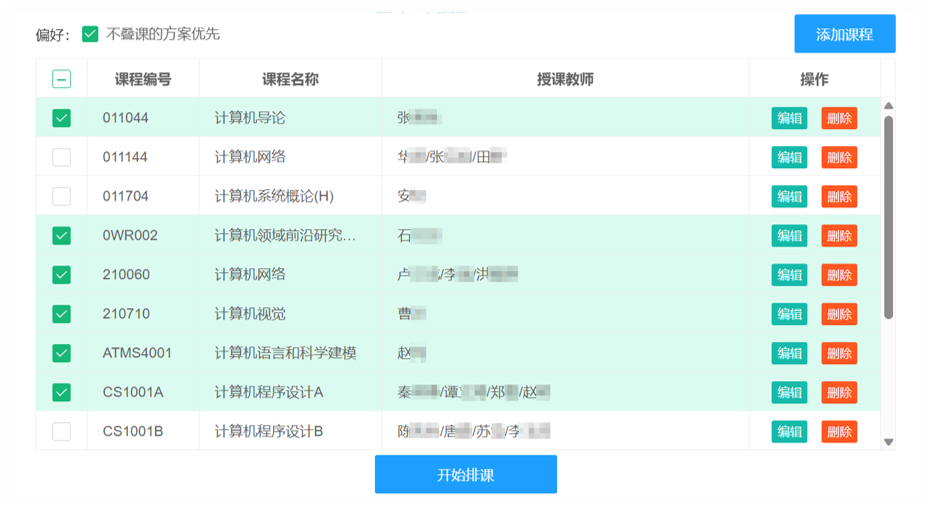
\includegraphics[width=\columnwidth]{figure/p1.png}
  \caption{蜗壳排课工具主页}
  \label{fig:p1}
\end{figure}

图 \ref{fig:p2} 展示了本工具的“添加课程”页面。在此页面,用户可以通过课程编号、课程名称、授课教师等信息来搜索课程,本网站已收录 2500 多个课堂,并定期自动从教务系统同步。额外地,我们引入了评课社区的课程评分,以供用户参考。添加课程时可以输入每个课堂的倾向度,工具将根据倾向度和课堂时间自动排课。

\begin{figure}[htbp]
  \centering
  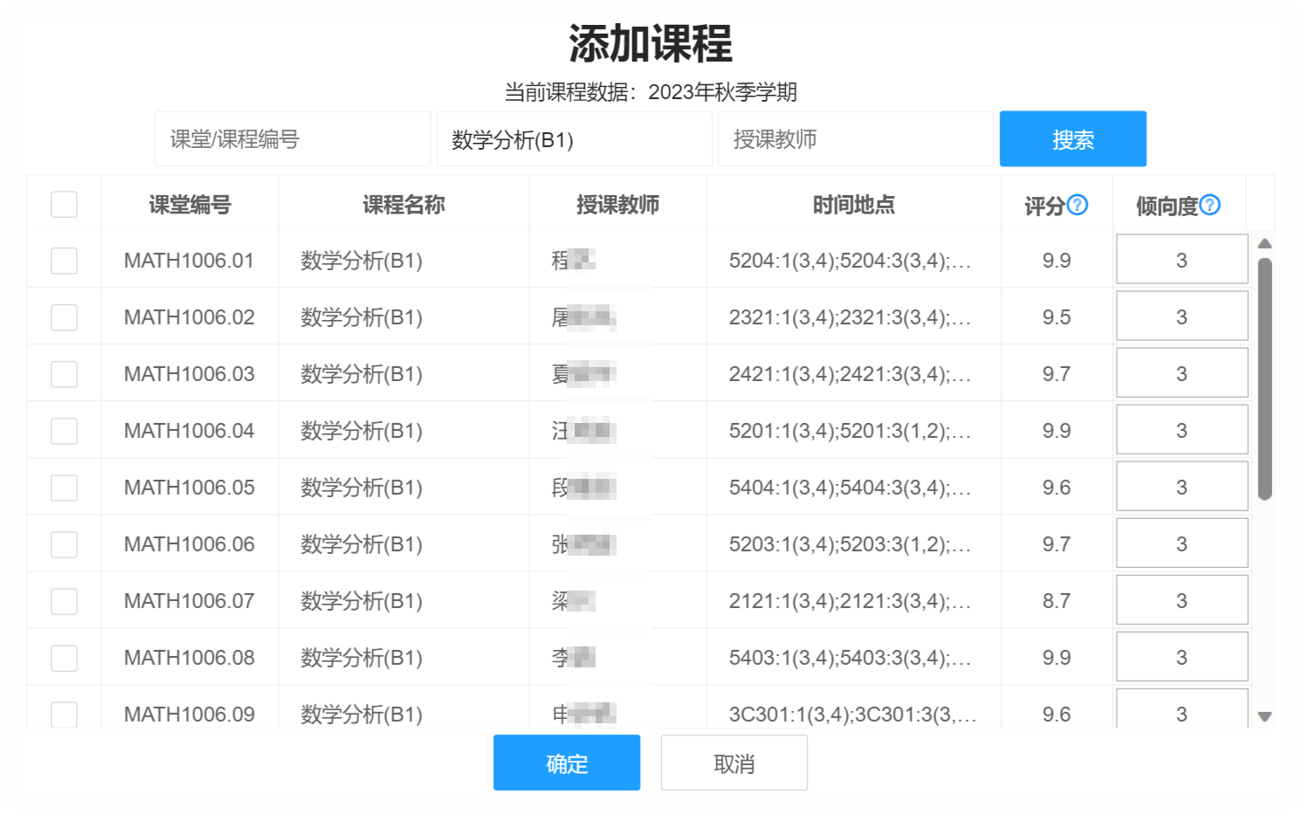
\includegraphics[width=\columnwidth]{figure/p2.png}
  \caption{蜗壳排课工具“添加课程”页面}
  \label{fig:p2}
\end{figure}

本工具呈现的排课方案,既有清晰的列表形式,也有直观的课程表形式。课程表样式与教务系统基本相同,但我们进行了样式的优化,使之更加清晰明了,且对小屏幕设备更为友好。

\subsection{我的科大}

我的科大包含教室查询、学校周边、校园导航等 34 项链接功能,以及任务清单、资料分享等 7 项自研功能,如图 \ref{fig:m1} 所示。然而,软件安装包仅有 \qty{2.5}{\mega\byte},安装后体积也仅 \qty{5}{\mega\byte},可谓“麻雀虽小,五脏俱全”。

\begin{figure}[htb]
  \centering
  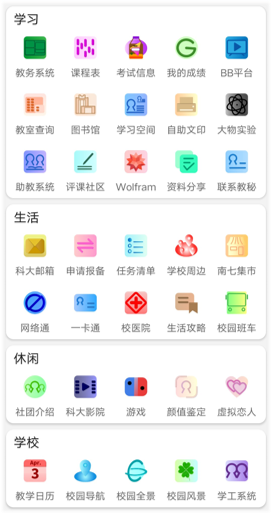
\includegraphics[width=0.67\columnwidth]{figure/m1.png}
  \caption{我的科大主页}
  \label{fig:m1}
\end{figure}

为了实现自动登录统一身份认证和科大邮箱,我的科大将密码加密存至本地,即便手机中潜藏病毒软件,也难以窃取信息,可谓“一夫当关,万夫莫开”。除了用于统计用户量、启动次数、版本分布等而收集的去敏化的设备信息外,我们没有将任何用户信息上传至服务器。即便如此,我们仍编写了 APP 隐私政策,APP 将严格按照该隐私政策保护用户的信息。
软件已完成了工信部 ICP 备案并放置备案号。反观市场上的软件目前几乎均未放置备案号,在这一点上,我们遥遥领先。此外,我的科大基于 Kotlin 语言开发,它是一门具有朝气和活力的语言。

细节决定成败。我的科大在图标、文本的布局、气泡提示、按钮位置等方面,均遵循人体工学设计。初次登录邮箱时输入的邮箱地址,我们贴心地预先加上了“@mail.ustc.edu.cn”,避免同学们——尤其是新生——遗漏或忘记输入“mail.”;当然,之后的每次登录,账号密码都会自动填充。积微成著,聚沙成塔,这些细节的精雕细琢,为用户带来了极致体验。

我们倾听用户的声音。一方面,APP 中设有反馈选项,用户可以通过填写问卷向我们反馈;另一方面,我们还通过用户交流群发布群投票,以不断优化我们的产品。我们采纳了用户的许多有益意见,例如实现了网页内文件下载功能,添加了“科大影院”功能,课程表添加了自定义课程的功能。我们始终将用户体验置于首要位置,不断创新,不断前行。

\section{测试、运行情况}

\subsection{测试情况}

本程序的每一个实验模块由组员完成后,组长会进行代码审核与测试,
如果发现问题则要求继续修改,直到所有问题被解决后该实验模块才会发布。
我们还建立了用户 QQ 群,并即时反馈用户提出的任何问题。

另一方面,各种 API 的编写与模块化编程也让我们的程序在编写过程中更不容易出错,
同时规范、统一的码风也让调试变得轻松。

\subsection{运行情况}

本项目从 2022 年 4 月 27 日上线以来,有超过 9000 次的浏览量,总访客数达到了 2100。

% \begin{figure}[htbp]
%   \centering
%   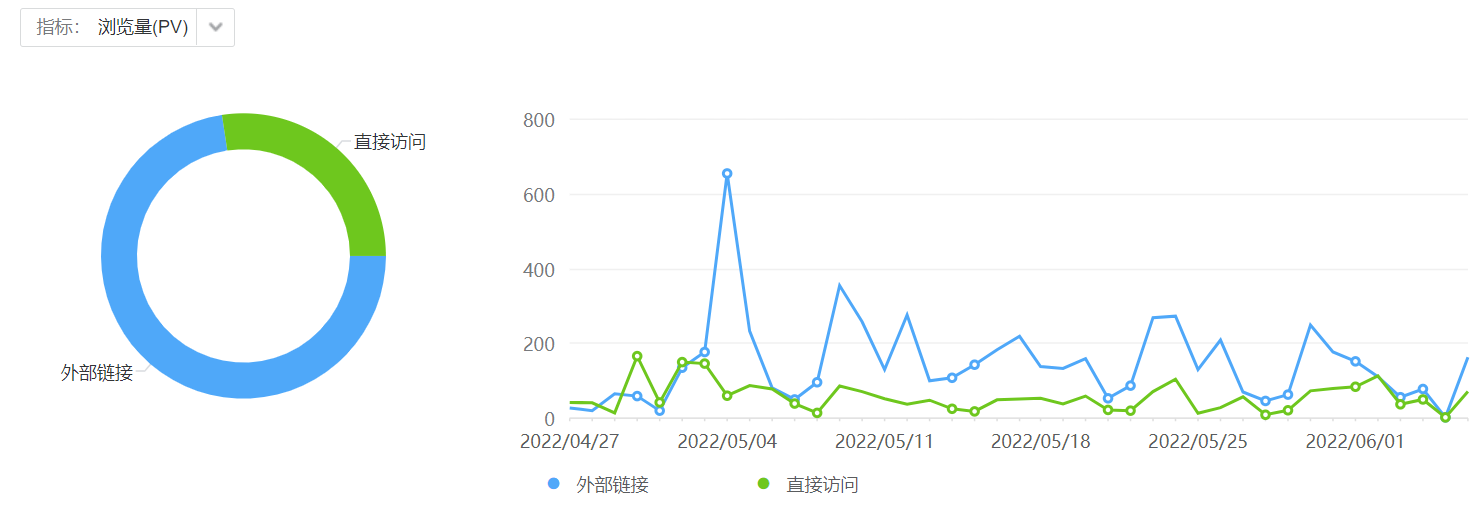
\includegraphics[width=\columnwidth]{figure/0.png}
%   \caption{4 月 27 日至 6 月 7 日的网站浏览量}
%   \label{fig:0}
% \end{figure}
% \begin{figure}[htbp]
%   \centering
%   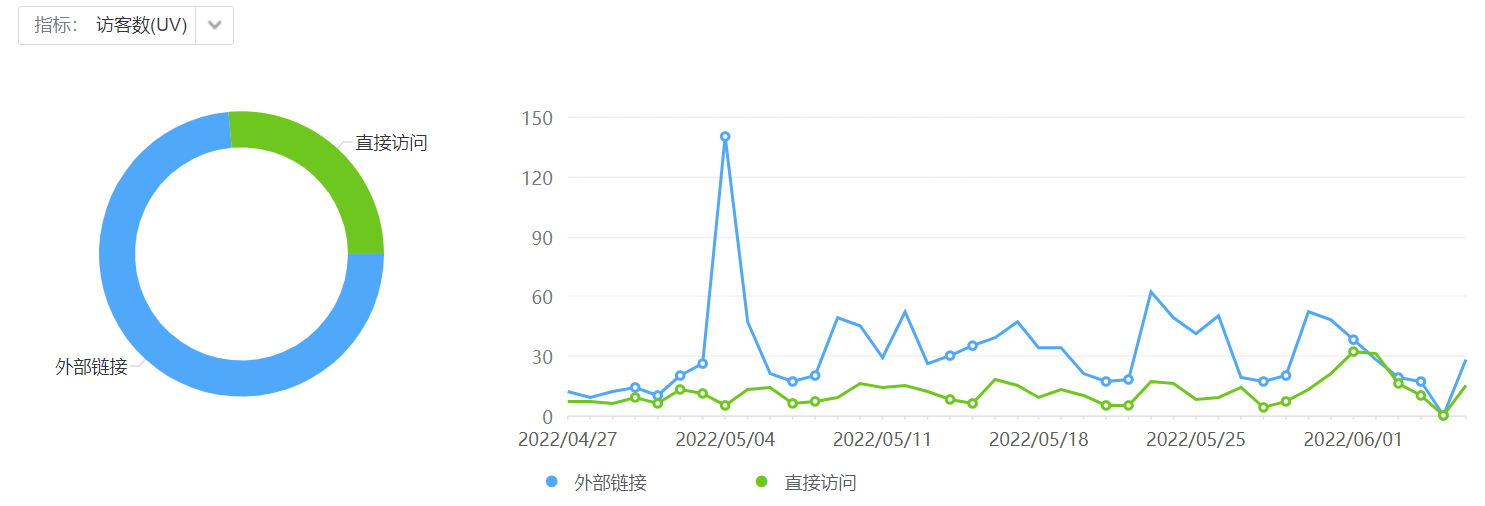
\includegraphics[width=\columnwidth]{figure/1.png}
%   \caption{4 月 27 日至 6 月 7 日的网站访客数}
%   \label{fig:1}
% \end{figure}

最后一次大物实验于 2022 年 6 月 3 日结束。
在大物实验结束之前,平均每天约有 50 名同学访问了我们网站,如图 \ref{fig:2} 所示。
考虑到每天只有不到 400 名大一学生做大物实验,本程序的使用率相对较高。
用户的平均访问时长为 6 分 36 秒,这说明我们的大雾实验工具非常简明易用。

\begin{figure}[htbp]
  \centering
  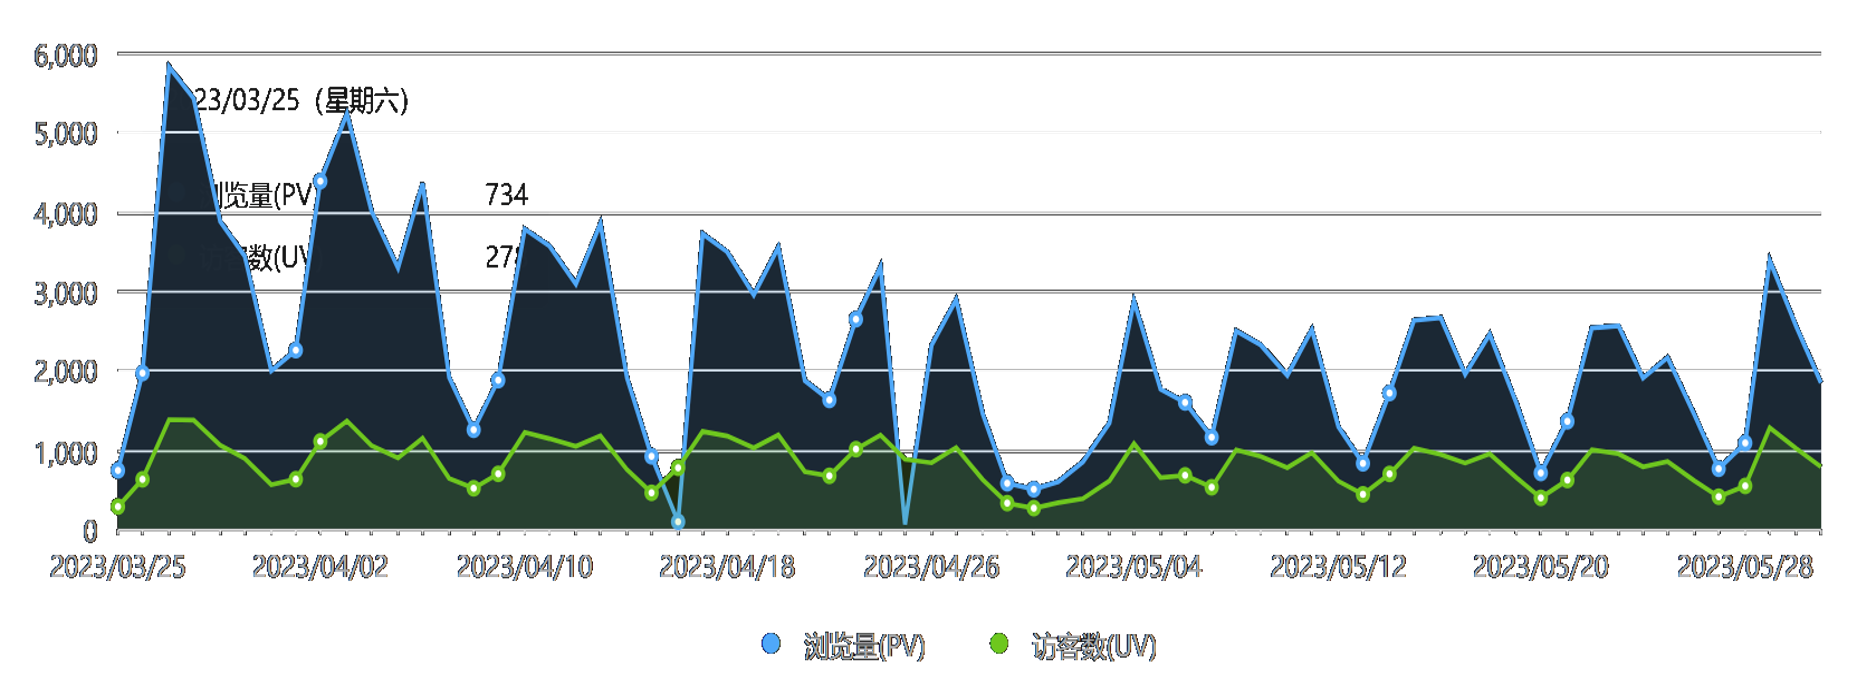
\includegraphics[width=\columnwidth]{figure/2.png}
  \caption{4 月 27 日至 6 月 6 日的统计数据}
  \label{fig:2}
\end{figure}
% \section{设计、开发过程中的难点}

鉴于我组成员都有一定的编程基础,整个项目中我们并没有遇到较大的困难,主要只有两个方面的小障碍:

第一,对实现的接口不够熟悉。由于我们编写的 API 参数较多,故未参与编写 API 的组员在一开始时需要花一点时间熟悉其调用方式。不过在后期大家也逐渐熟练地掌握了所有 API 的使用方式,而不用再去翻阅帮助文档。

第二,对物理实验本身不够了解。有的物理实验原理复杂、参考资料有限,且实验课程标准在不断变化,这会使程序生成的报告存在瑕疵,影响本项目的声誉。
% \section{小组分工}

\textbf{孙旭磊}:组织策划、前端与前后端衔接、数据处理 API 编写、公式插入 API 编写、数据处理示例程序编写、帮助文档编写、代码审查、海报和宣传片制作、实验报告修订,5 个实验处理模块的开发;\textbf{张学涵}:实验报告编写、数据处理 API 修订, 5 个实验处理模块的开发;\textbf{秦沁}:宣传推广、实验报告修订,4 个实验处理模块的开发;\textbf{赵奕}:技术与安全支持、实验报告修订,4 个实验处理模块的开发;\textbf{鲍政廷}:海报制作、实验报告修订,6 个实验处理模块的开发。具体的实验模块分工可参考本项目源码中的 \verb|README.md|。
\section{总结与展望}
\subsection{项目源码}
大雾实验工具源码和开发文档见\href{https://github.com/feixukeji/PhyX}{GitHub},蜗壳排课工具源码见\href{https://rec.ustc.edu.cn/share/58855c20-6911-11ee-946f-d117a7db9848}{此处},我的科大APP源码见\href{https://rec.ustc.edu.cn/share/1e33e8c0-6911-11ee-bd5b-631c3fa07e2e}{此处}。

\subsection{产品鲁棒性}
我们在开发过程中采取了有效的技术手段,使产品具有极佳的鲁棒性。无论胡乱输入什么东西,或者有意做任何非常规操作,我们的应用均不会奔溃。

\subsection{蜗壳作业助手}
除了上述三款已发布的产品外,我们还在筹划一款新的产品——蜗壳作业助手。

众所周知,我校布置作业的平台众多,各课程所用平台各异。若没能记住,便需要在QQ群消息、群文件、群公告、群作业、BB平台、瀚海教学网等各处寻觅。并且,作业完成数日后,又会忘记自己是否已完成、是否已提交,于是不得不又前往各个平台检查。

我们痛定思痛,计划打造一款统一的作业布置、提交平台,已完成和未完成的作业分别列表呈现。

不仅如此,我们将利用API自动获取以上各个平台的作业信息,使同学们免于繁琐的翻阅。当学生完成作业后,对于需要提交电子版的作业,直接提交在蜗壳作业助手上,助手将自动通过API同步提交到上述平台;对于需要上交纸质版的作业,可以在助手上做打钩标记,以便使自己记得确实完成了该作业。

我们已经完成了程序接口的设计,即将开始实现相应功能。

\subsection{生态融合}
我们这几款产品并非独立的产品,我们正积极推进生态融合。目前,大雾实验工具和蜗壳排课工具已集成至我的科大APP,这是生态融合的初步尝试。未来,我们将进一步融合,例如将我的科大APP的“任务清单”功能与蜗壳作业助手进行结合。

\subsection{团队协作}
我们分工明确,使用 git 进行协作,每个人的任务都有截止时间,这使我们的进度有序推进。以往的经历中,代码与相关工作往往都是独立完成,代码规范与项目进程完全由自己安排。但是在这种大工程中,相关代码需要符合规范,需要与队友交接,工作进度也要与队友进度相符。在这种分工体系下,每个人都要完成自己的任务,并顾及与他人的交互。

特别是大雾实验工具,我们建立了统一的码风,代码注释清楚,并制定了自主编写的 API 的详细使用说明。这样做一方面可以使得产品最终具有一致性——不同人写的代码能够基本一致;另一方面也使得最终的检验与调整能够更加方便——规范的代码提高了代码的可读性,降低了代码的审核成本。

\subsection{期待合作}
我们深知“一花独放不是春,百花齐放春满园”,“蜗壳365”秉持合作开放的态度,热切期待与其他同学的合作。

\section{致谢}
首先特别感谢余庆杯组委会为我们提供这样一个项目开发和展示的机会。

其次,在“蜗壳365”的开发与运维过程中,我们在视觉艺术、功能模块、宣传推广、意见反馈等方面得到了许多同学的帮助,列举如下:

苏宗山、秦沁、鲍政廷、周旭冉、尹冠霖、夏熙林、陈艺雨、陈思、王星河、蔡卓凡、施耀炜、李昊、邱梓惠、陈逸翀……

在此特别向他们表示衷心的感谢。如果获奖,我们会将奖金分予他们以表谢意。

同时,我们感谢广大用户对我们的支持和厚爱,我们将秉持初心,勇攀高峰,我们的“蜗壳365”将持续提供极致的免费服务。

% \section{参考资料}

\href{https://matplotlib.org/stable/index.html}{\texttt{Matplotlib}}, \href{https://pandas.pydata.org/docs/}{\texttt{pandas}}, \href{https://docs.scipy.org/doc/scipy/}{\texttt{SciPy}}, \href{https://docs.sympy.org/latest/index.html}{\texttt{SymPy}}, \href{https://python-docx.readthedocs.io/en/latest/}{python-docx} 等包的使用方法参考了官方文档,
遇到的各种问题则是查阅 \href{https://stackoverflow.com/}{Stack Overflow} 等网站上的讨论。
在 Word 中渲染 \LaTeX{} 公式的方法,参考了 \verb|python-docx| 开源仓库里一份 Github Issues 中提出的\href{https://github.com/python-openxml/python-docx/issues/320#issuecomment-798749198}{解决方案}。

\vskip 0.05in
{\noindent\large\bfseries 另附}
\begin{itemize}[nosep]
  \item 大雾实验工具网址:\url{https://dawu.feixu.site/}
  \item 宣传片地址(发布于 B 站):\url{https://www.bilibili.com/video/BV193411G7aP}
  \item 项目源代码(文件目录见其中的 \verb|README.md|)
\end{itemize}
% \printbibliography[title=参考文献]
% \appendix
\onecolumn
\section{Appendix}

\begin{center}
  \fbox{\LARGE 此页不打印}
\end{center}

未完成:
斜率计算过程的 \LaTeX{} 与 \verb|MathML| 代码,
截距与 Pearson's r 的计算公式错误,
最终结果有效位数:不确定度应只有 1 位。

\end{document}